\documentclass[titlepage]{scrartcl}
\usepackage[ngerman]{babel}
\usepackage[T1]{fontenc}
\usepackage[utf8]{inputenc}
\usepackage{graphics}
\usepackage{graphicx}
\usepackage{tikz}
\usetikzlibrary{shapes.misc, positioning, shapes.multipart}
\usepackage{placeins}
\usepackage[dvipsnames]{xcolor}
\usepackage{hyperref}
\usepackage{caption}


\titlehead{Wintersemester 2023/24}
\title{\TicTacToe}
\subtitle{Dokumentation der Evaluationsstrategien}
\date{Stand: \today}
\author{Jonas, Luis, Leonid}

\newcommand{\TicTacToe}{TI\reflectbox K Tac Toe}

\begin{document}
\maketitle

\emph{Hinweis:} Aufgrund der besseren Lesbarkeit ist in diesem Dokument nur von Spielern und Nutzern die Rede.
Es sind aber immer Spielerinnen und Spieler und Nutzerinnen und Nutzer aller Geschlechter gemeint.

"`Spieler"' meint im Folgenden immer die Entität, die eine der beiden Positionen im Spiel Tic-Tac-Toe (Kreuz oder Kreis) übernommen hat.
Die Person, die die App benutzt, wird "`Nutzer"' genannt.
\section{KI-Elimination}
Die einfache Eliminationsstrategie ist eine Evaluationsstrategie, welche den KIs aus \TicTacToe{} nativ zugeordnet werden kann.

Beim Erzeugen der KI sind die Gewichte der KI vollständig auf "`1"' gesetzt (siehe Abbildung \ref{eliminationPrä}).

Bei dieser wird am Ende eines Spiels das Gewicht des letzten Zuges des Verlierers (egal ob die KI verloren hat oder nicht) auf \glqq{}0\grqq{} gesetzt.
In Abbildung \ref{eliminationPost} kann die Änderung für ein typisches erstes Spiel nachvollzogen werden.

Danach werden alle Gewichte der Züge des gerade absolvierten Spiels überprüft. Dabei wird überprüft, ob es einen Spielzustand gibt, bei dem ein Spieler in Zukunft nur Züge mit Gewicht 0 machen kann.
Falls dem so ist, wird auch das Gewicht des davor vom betreffenden Spieler getätigten Zuges auf \glqq{}0\grqq{} gesetzt.
Dies wird jedes Mal sowohl für die Züge der KI als auch für die Züge ihres Gegners durchgeführt.
In Abbildung \ref{elimination1} ist ein Beispiel zur Veranschaulichung zu sehen.

Falls es ein Unentschieden gab, werden keine Gewichte geändert. 

\begin{figure}[htb]
\includegraphics[width = \linewidth]{eliminationPrä.png}
\caption{Gewichte der Eliminations-KI nach einem typischen ersten Spiel, vor dem Anwenden der Evaluationsstrategie}
\label{eliminationPrä}
\end{figure}
\begin{figure}[htb]
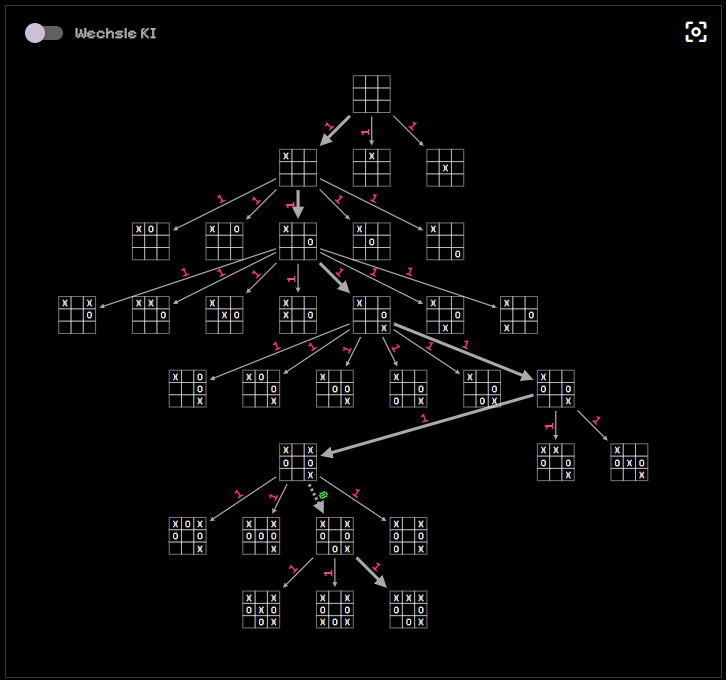
\includegraphics[width = \linewidth]{eliminationPost.png}
\caption{Gewichte der Eliminations-KI nach einem typischen ersten Spiel, nach dem Anwenden der Evaluationsstrategie}
\label{eliminationPost}
\end{figure}

\begin{figure}[htb]
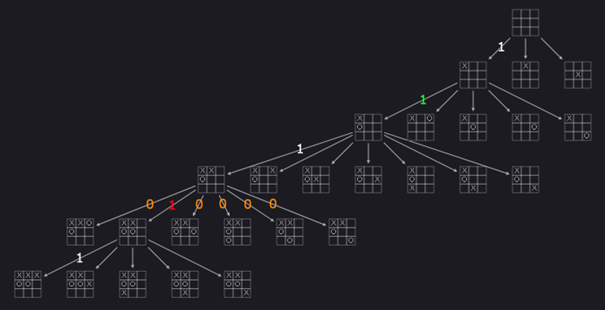
\includegraphics[width = \linewidth]{elimination1.png}
\caption{Die Strategie Elimination ändert Gewichte weiter oben im Baum}
\label{elimination1}
\end{figure}

Angenommen wir haben ein Spiel zwischen einem Menschen (X) und einer Eliminations-KI (O).
Der menschliche Spieler ist zuerst am Zug.
Die Gewichte der KI könnten wie in Abbildung \ref{eliminationPrä} aussehen.

Wird in diesem Fall die Belohnung der Eliminations-KI durchgeführt, wird zuerst die vorletzte hervorgehobene 1 auf 0 gesetzt, da dies den letzten Zug des Verlierers beschreibt.
Denn der Verlierer hat damit dem Gegner erlaubt einen Zug zu machen, welcher diesen gewinnen lässt.
Das Ergebnis davon ist in Abb.~\ref{eliminationPost} zu sehen.
Nach einigen Spielen könnten die Gewichte aussehen wie in Abbildung \ref{elimination1}.
Dort wurde überprüft, ob es Spielzustände gibt, von denen aus es nur 0-Gewichte gibt. Da die vorletzte 1 zu einer 0 geändert wurde, sind von dem Spielzustand darüber nur Züge mit Gewicht 0 möglich. Aus diesem Grund wird die vorhergehende 1 auch auf 0 gesetzt. Denn falls der grüne Zug von einem Spieler gespielt wird, kann sein Gegner mit einem Zug antworten, sodass dem Spieler nur noch Züge, welche mit 0 markiert sind bleiben.

Hinweis: Angenommen, die Rollen wären bei gleichem Spielverlauf vertauscht, die KI hätte also das Zeichen X, sie hätte angefangen zu spielen und hätte gegen den Menschen gewonnen, würden sich die Gewichte der KI genauso ändern, da sie auch von den Zügen des Gegners lernt.
\FloatBarrier
\newpage

\section{KI-Elimination v2.0}
Die verbesserte Eliminationsstrategie ist eine Evaluationsstrategie, welche den KIs aus \TicTacToe{} nativ zugeordnet werden kann.

Sie wird für Verlustzüge und Unentschieden gleich belohnt wie die einfache Eliminationsstrategie.
Allerdings berücksichtigt sie zusätzlich \emph{Gewinnzüge}.
Ein Gewinnzug ist ein Zug, der (aus Sicht der KI) den Gegner dazu zwingt, einen Zug zu wählen, der mit "`0"' gewichtet ist.
Einen solchen Gewinnzug wählt die verbesserte Eliminations-KI immer aus und setzt dafür alle Alternativen zum Gewinnzug auf Gewicht 0.
In Abbildung \ref{elimination2} ist beispielsweise der letzte Zug ein Gewinnzug, daher werden die beiden anderen Züge auf 0 gesetzt.
Es ist zu beachten, dass dies auch einen anderen Gewinnzug löscht.

\begin{figure}[htb]
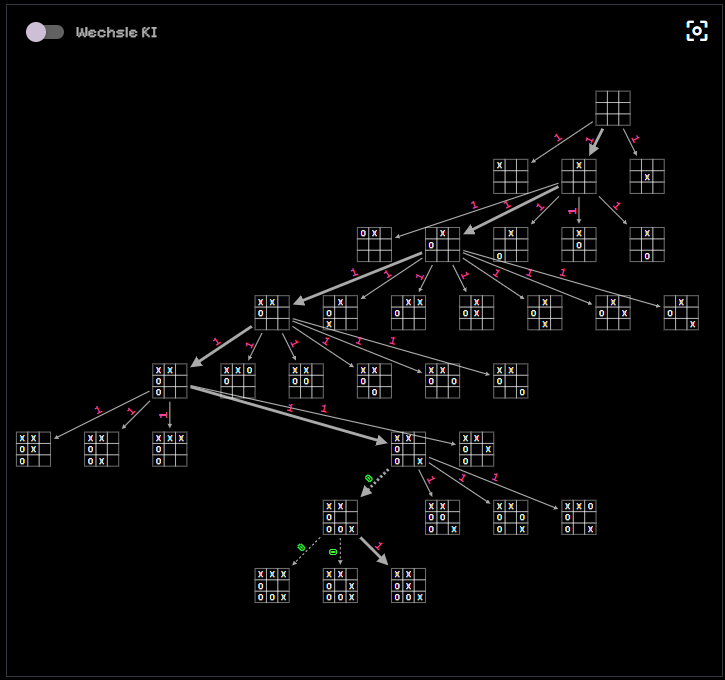
\includegraphics[width = \linewidth]{elimination2.png}
\caption{Die Strategie Elimination v2.0 ändert Gewichte bei Gewinn}
\label{elimination2}
\end{figure}

\FloatBarrier
\newpage
\section{KI-Rückführung}
Die Rückführungsstrategie ist eine Evaluationsstrategie, welche den KIs aus \TicTacToe{} nativ zugeordnet werden kann.

Beim Erzeugen der KI sind die Gewichte der KI auf "`\(9-\textrm{H\"ohe}\)"' gesetzt (siehe Abb.~\ref{rückführungPrä}).

Es kann manuell gesetzt werden, welche Zahlen bei Gewinn, Verlust und Unentschieden auf die bestehenden Gewichte der KI addiert werden (diese dürfen auch negativ sein).
Das entsprechende Menü ist in Abbildung \ref{rückführungEinstellungen} zu sehen.
Die Gewichte werden jedoch niemals negativ.

Am Ende eines Spiels werden alle Gewichte der Kanten, die tatsächlich gespielt wurden (hervorgehoben und orange in Abbildung \ref{rückführungPrä}), mit den vorgegebenen Vorschriften verändert (siehe Abb.~\ref{rückführungPost}).

\begin{figure}[htb]
\centering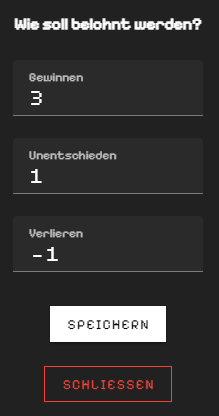
\includegraphics{rückführungEinstellungen.png}
\caption{Die Einstellungen für Rückführungs-KIs}
\label{rückführungEinstellungen}
\end{figure}

\begin{figure}[htb]
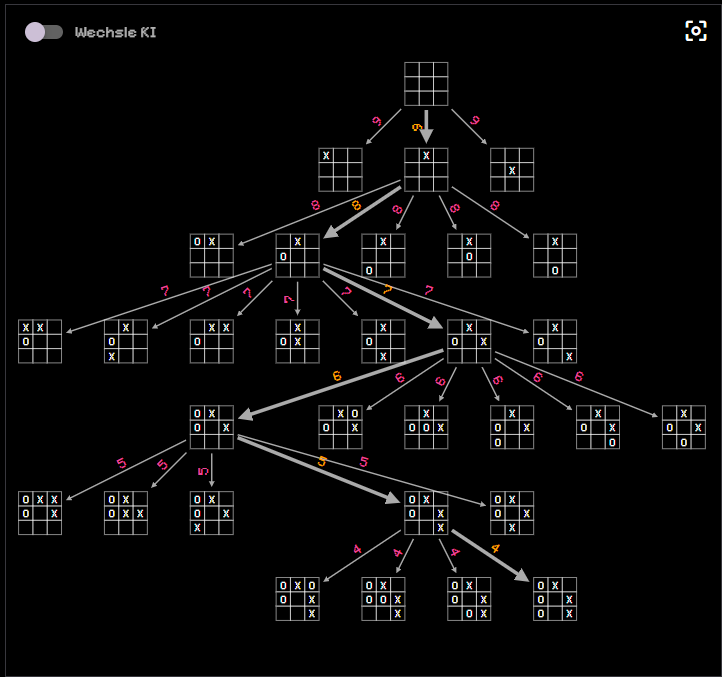
\includegraphics[width = \linewidth]{rückführungPrä.png}
\caption{Gewichte der Rückführungs-KI nach einem typischen ersten Spiel, vor dem Anwenden der Evaluationsstrategie}
\label{rückführungPrä}
\end{figure}

\begin{figure}[htb]
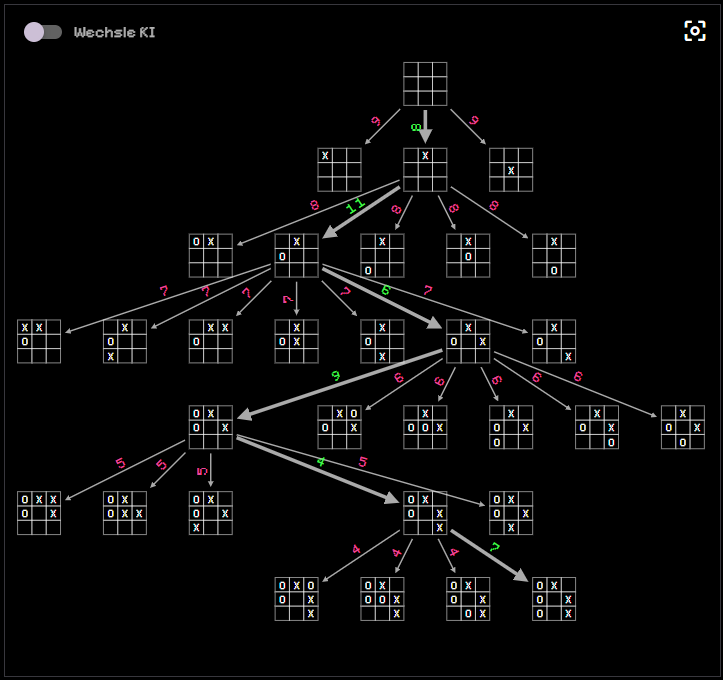
\includegraphics[width = \linewidth]{rückführungPost.png}
\caption{Gewichte der Eliminations-KI nach einem typischen ersten Spiel, nach dem Anwenden der Evaluationsstrategie}
\label{rückführungPost}
\end{figure}

\end{document}























